\newtheorem{uwaga}{Uwaga}

\newtheorem{lemma}{Lemma}
\newtheorem{deff}{Definition}

\section{Juliusz Kociński}
\subsection{SecuRank Dependency Grading System [ENG]}
\begin{center}
The following is the overview of the \textbf{SecuRank }Dependency Grading Model created for the 2020 Goldman Sachs Warsaw Hackathon.\\ 
\large A method of giving a security ranking for dependencies based on their metadata.
\\

\normalsize

    This is short overview of the method used to determine a "safety rank" to packages included in a software project in a SecuRank system.
    Part of project created during Goldman Sachs Warsaw Hackaton.
\end{center}

\hline

\normalsize

\subsubsection{Main concept}
At first Let's define main function giving a rank to each dependency or the entire project. We will judge the security based on the (finite) number of factors. We'll focus on them later. Let's define our strategy:
Let $d$ be a "main" package (or a project) such a:

$A_d = \{d_i | i \in \mathbb{N}, d_i \in D,  d_i$ is a dependency of $d \}$ - Set of dependencies of $d$.\\
That means that for example $d_{2,3}$ is a "3rd" dependency of a "2nd" dependency of $d$. $D$ is a set of all dependencies. Also Let ${A'}_d$ be a set of all of the dependencies of elements of set $A_d$. In other words ${A'}_d = \{ e_j | e\in \bigcup_{j=1}^{k} A_{d_j} \} $. Remember, every ${A'^{n}}_d$ with ${A'^{(n-1)}}_d$ is in the same relation as $A'_d$ with $A$.
\\
Then we have set of marking functions:\\
Let $F_j:~D \rightarrow [0,1]$ be a function that takes dependency $d \in D$ and ranks it in scale from 0 to 1 based on a well defined factor $j$. These factors include for example update regularity and publisher. Now we can finally define our dependency-grading functions:
\begin{itemize}
    \item First, single dependency grading function:
    \begin{deff}
    $R(d):=  \frac{ \sum_{j=1}^n {\alpha_j F_j(d)} }
            { \sum_{j=1}^n {\alpha_j}}$
    \end{deff}
    
    \item Then final score considering entire dependency tree:
    (note: second definition is recursive but much more clear) 
    \begin{deff}
    $
     G(d):= min( \frac{R(d_0)}{x^0}, 
           \frac{R(d_1)}{x^1}, \frac{R(d_2)}{x^1}, ... , \frac{R(d_n)}{x^1},
           \frac{R(d_{1,1})}{x^2}, ... ,\frac{R(d_{n,m})}{x^2}, ... )\\
     G(d):=
        \begin{cases*}
          R(d) & \leftarrow |A_d| = 0 \\
          min( R(d), \frac{G(d_1)}{x}, \frac{G(d_2)}{x}, ... , \frac{G(d_n)}{x} )   & \leftarrow |A_d| = n \neq 0
        \end{cases*}
    $
    \end{deff}
    
\end{itemize}
%Usunięcie dolara powoduje bugi. Tak zgłasza błąd, ale działa 
\subsubsection{Grading factors}
Now Let's focus on one of these functions $F_j(d)$ we mentioned earlier:

\textbf{}{Update regularity}
Lets define out function for grading update regularity $F_u:D \rightarrow [0,1]$:

Making long story short, timestamp $t$ is a number representing some point in time let's define $t_n = t_1, t_2, ... , t_n$ as a chronological sequence of timestamps of all the different version of the package. We'll use $c$ which is some period of time. If the period between updates is shorter than $c$ it satisfies us and package get a full rank. Most recent updates are more important.\\
Therefore:
\begin{deff}
\Large $F_u(d) = \frac{2 \sum_{i=1}^{n-1} \frac{i}
                         {1+max((t_{i+1}-t_i)-c, 0)}}
         {n(n-1)}$
\end{deff}
\hline


\subsection{Plan sieci w budynku [PL]}
{\uwaga
    Tablice małych routerów - z access pointami (czyli routerów podsieci pojedynczych sal/pokojów) nie są ukazane ze względu na wyjaśniające to schematy i ich olbrzymią ilość. Ich tablice są dość łatwe do wywnioskowania ze schematów w \ref{fig:budA}
    }
\begin{enumerate}
    \item Schemat sieci w budynku A:
    (schemat znajduje się na następnej stronie dla czytelności)
    
    \begin{sidewaysfigure}[h!]
        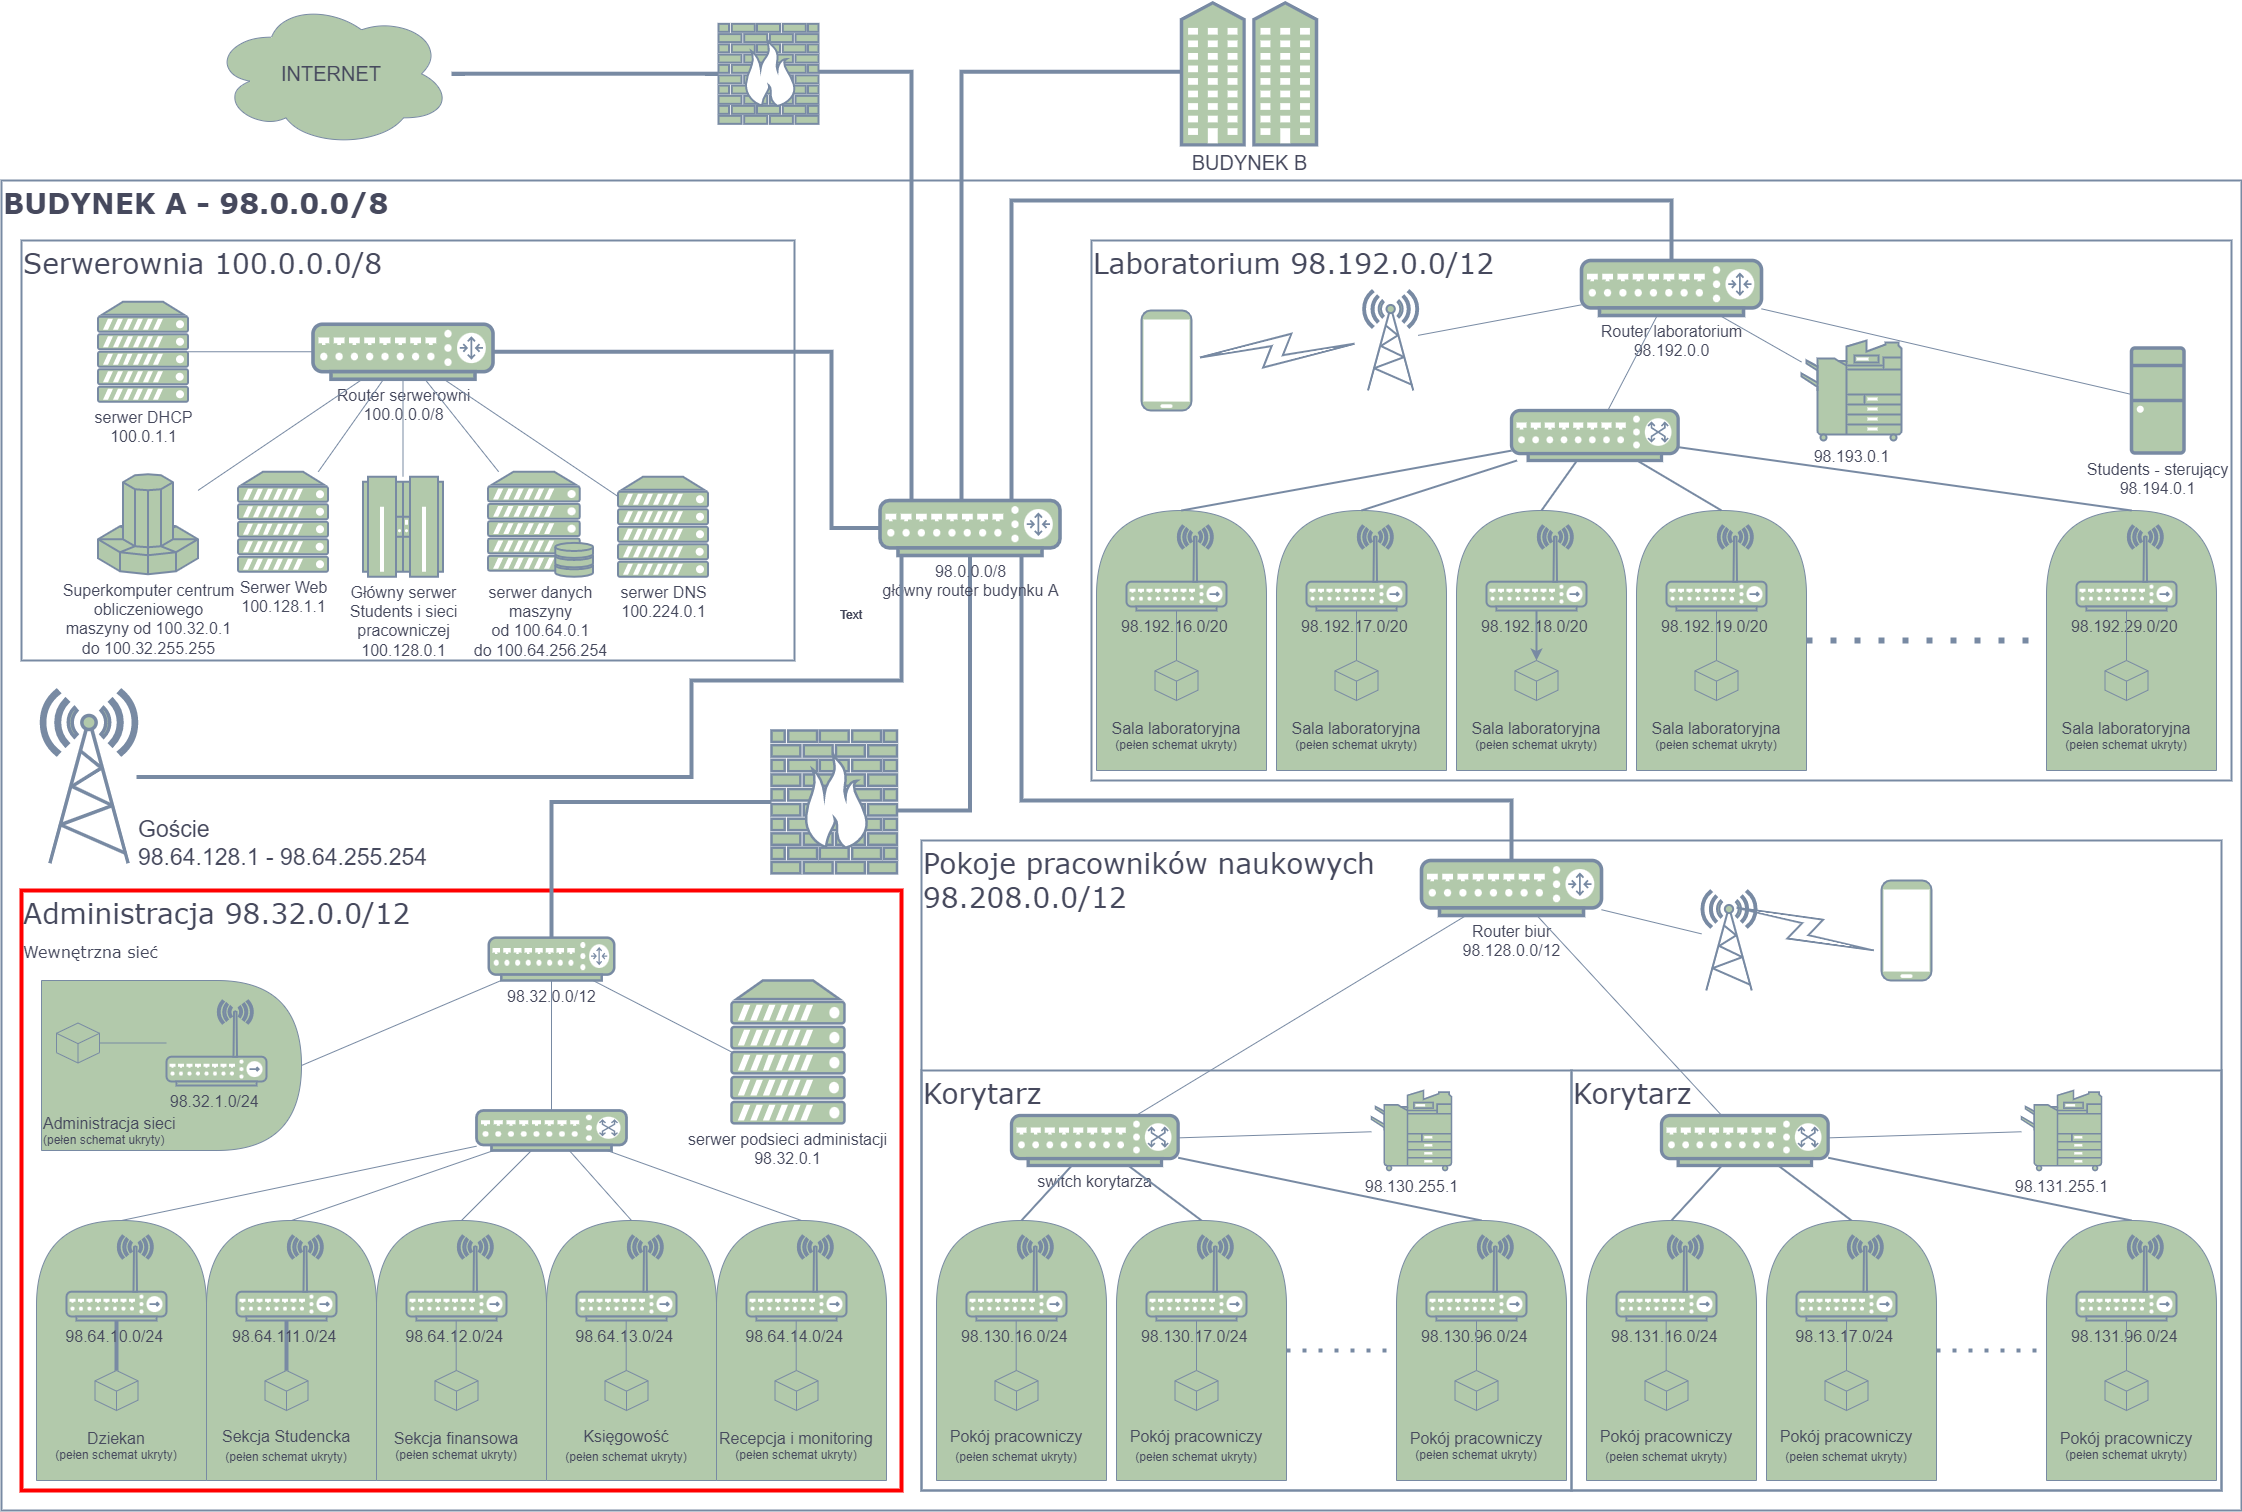
\includegraphics[
            width = 1\textwidth,
            height = 1\textheight,
            keepaspectratio
        ]{pictures/budynekA.drawio.png}
        \caption{Schemat sieci w budynku A}
        \label{fig:budA}
    \end{sidewaysfigure}    

    \item Tablica tras budynku A:\\
\begin{tabular}{|c|c|c|c|}
    \hline
        \multicolumn{4}{|c|}{\textbf{główny router budynku A}} \\
    \hline
        sieć & maska & brama & interfejs \\
    \hline
        \multicolumn{4}{|c|}{(w przypadku awarii połączenia z routerem A:)} \\
        0.0.0.0     &   0.0.0.0         &   96.0.0.0    &   eth1    \\
        98.0.0.0    &   255.0 0 0       &   0.0.0.0     &   eth1    \\
    \hline
        \multicolumn{4}{|c|}{(Gdy wszystko działa:)} \\
        0.0.0.0     &   0.0.0.0         &   193.1.42.1  &   eth0    \\
        193.1.42.0  &   255.255.255.0   &   0.0.0.0     &   eth0    \\
    \hline
        100.0.0.0   &   255.0.0.0       &   0.0.0.0     &   eth1    \\
        96.0.0.0    &   255.0.0.0       &   0.0.0.0     &   eth2    \\
        98.32.0.0   &   255.240.0.0     &   0.0.0.0     &   eth3    \\
        98.64.0.0   &   255.240.0.0     &   0.0.0.0     &   eth4    \\
        98.128.0.0  &   255.240.0.0     &   0.0.0.0     &   eth5    \\
        98.192.0.0  &   255.240.0.0     &   0.0.0.0     &   eth6    \\
    
    \hline
    
%\label{tab:netA}
\end{tabular}
\end{enumerate}